\documentclass[]{article}
\usepackage[utf8]{inputenc}
\usepackage[spanish]{babel}
\usepackage{graphicx}
\usepackage{vmargin}

\setpapersize{A4}
\setmargins{2.5cm}       % margen izquierdo
{1.5cm}                        % margen superior
{16.5cm}                      % anchura del texto
{23.42cm}                    % altura del texto
{10pt}                           % altura de los encabezados
{1cm}                           % espacio entre el texto y los encabezados
{0pt}                             % altura del pie de página
{2cm}                           % espacio entre el texto y el pie de página

%opening
\title{Apuntes para preparar \textsc{Green Belt}}
\author{Nicolás Rodríguez Lucena}

\begin{document}

\maketitle

\part*{Introducción}
\section{Six Sigma y metas organizativas}
Motorola fomenta el Six Sigma a finales de los 80. General Electric de primeras se muestra reticente pero en los 90 le mete mano. 

El fracaso más común es la falta de compromiso por parte de la dirección con la mejora real de los procesos.

\textit{Advanced quality planning (AQP)} para preparar para la implementación de un desarrollo Six Sigma con facilidad, mediante data-driven decisions. 

El especialista en \textit{Quality Control/Quality Assurance (QC/QA)} ha asegurado que los estandares eran establecidos y mantenidos para la satisfacción del cliente. La evolución llevo a apartar al experto QC/QA y darle toda la responsabilidad de la satisfacción de cliente en vez de ser incluida en todos los miembros de la organización. 

\textbf{Shewhart} utilizó gráficos para monitorizar procesos y detectar causas especiales que desviaran los resultados de lo esperado (\textit{quality control charts, process behavior charts}). \newline
Ford en 1988 lanzó el programa \textit{supplier quality improvement (SQI)} para trabajar con proveedores externos en nuevos diseños de vehículos utilizando los \textit{advanced quality planning (AQP)} de la ASQ para mejorar la calidad en el ensamblaje, todo esto dio lugar al \textit{advanced product quality planning (APQP)} que se utiliza en la industria automotriz. 

Motorola le presentó el Six Sigma a Ford y lo evaluó contra Ford Q1 y Q-101 (precursor de ISO/TS 16949). Solo un punto que no le gustó, estaba establecido el $C_p$ en 1.0. Ford quería $C_{pk} >$ 1.33 para procesos conocidos y $C_{pk} >$ 1.67 para los nuevos.

Six Sigma: reducir la variación y mejorar el control del proceso. Lean: expulsa residuos y promueve el estandarizar trabajos. 

\textbf{Subir Chowdhury}: los problemas pueden ser evitados a través de la mejora continua, la calidad es responsabilidad de todos los individuos, la calidad empieza arriba, todos tienen un papel en la calidad, la calidad es el balance entre el poder de la gente y del proceso. Poder de la gente necesita compromiso, honestidad y empatía. Process power es solucionar problemas, desarrollar ideas y soluciones. Toda organización es única, cada individuo trae diferente conocimiento y habilidades. Métodos y procesos deben ser desarrollados para cada específica situación.

\textbf{Philip Crosby}: Sus 14 pasos. 1) Gerencia comprometida con la calidad 2) Equipos de mejora continua con miembros de todos los departamentos 3) Determinar como medir donde están los problemas 4) Evaluar el coste de calidad 5) Incrementar la conciencia de calidad en la organización 6) Tomar acciones formales para corregir problemas identificados en pasos anteriores 7) Poner un comité de 0-defectos 8) Formación para todos 9) Establecer el día "cero defectos" 10) alentar a que la gente establezca metas de mejora para ellos y para sus grupos 11) alentar a la gente a que comente los problemas de gestión 12) reconocer y apreciar la participación de la gente 13) establecer "Consejos de Calidad" para comunicarse de manera regular. 14) Re-run el programa desde 0, para que la gente vea que esto nunca se acaba. 

\textbf{W. Edwards Deming}: Otros 14 puntos. 1) constancia en la mejora 2) nueva filosofia 3) no todo es inspección 4) no todo es precio 5) mejora constante para planificación, producción y servicio 6) formacion 7) liderazgo 8) evitar miedos 9) quitar barreras entre el staff 10) fuera el trabajo duro 11) quitar ránkins y mierdas para cuantificar trabajo duro y metas de gestión 12) quitar barreras que roben a la gente el orgullo del trabajo. Sistemas de méritos etc.. 13) Plan de Formación y mejora personal 14) Todos para realizar el cambio. Y sus 7 enfermedades mortales: 1) falta de constancia 2) el cortoplacismo 3) evaluacion por meritos y mierdas 4) Movilidad de la direccion 5) el funcionamiento basado solo en 'figuras visibles' 6) costes medicos excesivos 7) jugar en el borde de la ley. 

También preparó el \textit{Sistema del conocimiento profundo}: 1) Apreciación de un sistema (process aproach) 2) Conocimiento de la variación (existe, como reconocerla). 3) Teoría del conocimiento (how to learn) 4) Conocimiento de la psicología (Maslow, Regla de Platino...) 

\textbf{Armand Feigenbaum}: Planifica y transmite el plan. Planificar es bien ya que el propósito de la planificación es 'hacerlo bien'. En tres pasos: Liderazgo de la calidad, tecnología moderna de la calidad y comité de organización. Los planes AQP son suyos. 

\textbf{Kaoru Ishikawa}: Diagrama causa-efecto. Trabajó con Deming a tope. Sus puntos: Calidad primero, por delante de rentabilidad corto placista. Orientar hacia cliente (pensar desde su POV). El siguiente proceso es el cliente (que haya feedback). Hechos y datos, estadística. Humanidad como filosofía de gestión. Gestion interfuncional. 

\textbf{Joseph M Juran}: quality planning, quality control y quality improvement. Sus puntos: crear conciencia, la calidad es de todos, haz una infraestructura de calidad (council, appoint teams, ...), formación sobre Calidad, revisiones periodicas, reconocimiento a los equipos ganadores, revisar el sistema de recompensas para hacer cumplir el ratio de mejoras, mantener un plan de negocio basado en la mejora de la calidad. Pareto es suyo. 

\textbf{Dorian Shainin}: ing. aeronautico que desarrolla soluciones para los problemas mas dificiles. Habla con las \textit{parts}, son mas listas que los ingenieros. Invento la Red X.

\textbf{Walter Shewhart} trabajador de Western Electric inventó el PDCA y es el padre del control estadístico de proceso. 

\textbf{D. H. Stamatis}: 45 libracos sobre Six Sigma, calidad y demás. El Manual del FMEA es suyo y la documentación del Six Sigma.

\textbf{Genichi Taguchi}: Inventó la Loss Function, usada para medir el coste financiero por empeorar la calidad y desarrolló la filosofía de \textit{off-line quality control}. 

\textbf{Proceso}: serie de pasos diseñada para producir productos o servicios. A menudo representado como un diagrama de flujo con inputs (materiales, recursos, info), steps, y hay un output. Para aplicar Six Sigma, se meten los pasos del DMAIC (\textit{define, measure, analyze, improve y control}). 

\textbf{Business Systems}: diseñados para implementar un conjunto de procesos. Se asegura de que todo esté en el lugar adecuado en el momento adecuado. Tiene como meta la mejora continua de proesos, productos y servicios. Se encarga de recoger y analizar la información de los procesos y de otras fuentes para la mejora continua.  

Hay dos maneras de ver el método utilizando inputs / recursos para producir resultados de calidad: la gestión de procesos es recoger datos y analizarlo, aplicando el feedback al proceso. Por otro lado se piensa que el proceso debe ser diseñado orientado hacia la colección de datos, análisis y el feedback que se va a producir.

Man, Machine, Methods, Mother Nature, Management, Materials, Measurement System para Productos y/o Servicios.

Métodos alternativos al Six Sigma: Quality Operating System (QoS), mejora contiuna (CI), total quality management (TQM), mejora de procesos (PI), Reto: revisar procesos para mejoras: mantenimientos preventivos, limpieza, desgaste...

La línea general es: qué medir, cómo medirlo, es fundamental el proceso?, consenso sobre defectos, exponer defectos latentes, observar la calidad estadística (cartas de comportamiento de proceso), distinguir entre Calidad de Diseño y Calidad de Conformidad. 

\subsection{Modelo DMAIC}
Define: PDCA, SIPOC, 5W, Systems thinking, Process Identification, Flowchart, Project Management. \newline
Measure: PDCA, Data collection plan, Measurement systems analysis (MSA), Collect Data (check sheets, histograms, pareto charts, scatter diagrams), identificar variabilidad-instabilidad, benchmark, start cost of quality. \newline
Analyze: PD\textbf{S}A, mejora continua, mantenimiento preventivo, limpieza, benchmark, teorema del limite central, GD\&T, shop audit, experimentos. \newline
Improve: PD\textbf{S}A, mejora procesos, desarrollo organizacional, reducción de la variación, solución de problemas, brainstorming, flowchars 'should be', FMEA, coste de calidad, diseño de experimentos. \newline
Control: SDCA, plan de control, dynamic control plan (DCP), MSA largo plazo, mistake-proofing, process behavior charts.

\subsection{Six Sigma Road Map}

\begin{enumerate}
	\item Existe la variacion en todo. Hay que estandarizar el trabajo.
	\item Identifica lo que el cliente quiere y necesita. Reduce variación.
	\item Metodo problem-solving para mejorar los planes.
	\item Seguir el DMAIC para desarrollar la mejora.
	\item Monitorizar el proceso con Process Behavior Charts.
	\item Subir de nivel el estandar de los procedimientos y lecciones aprendidas.
	\item Celebrar el exito
	\item Empezar de nuevo con la mejora continua PDSA/SDCA.
\end{enumerate}

\subsection{Cost-Benefit Analysis}

Muchas cosas que funcionan en una tienda se pueden clasificar en: \textit{prevention cost}, appraisal costs (evaluacion), costes de fallos internos y costes de fallos externos. 
Cuando se calculan los costes de calidad en un negocio se plotea una curva tal como Fig \ref{fig:CurvaCostesdeCalidadInicio}.
\begin{figure}[ht!]
\centering
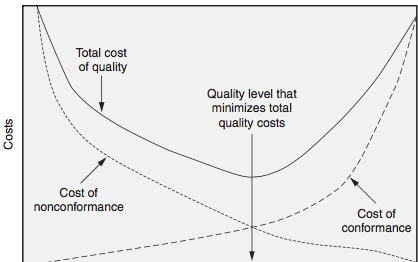
\includegraphics[width=90mm]{imagenes/CurvaCostesCalidadInicio.png}
\caption{Curva de Costes de Calidad antes de iniciar el desarrollo}
\label{fig:CurvaCostesdeCalidadInicio}
\end{figure}

En la primera ronda de medidas de costes nadie debe ser increpado, debe servir a modo comparativo y para sacar el qué hacer y el cómo hacerlo. La meta es intentar llegar a la Fig \ref{fig:CurvaCostesdeCalidadFin}.

\begin{figure}[ht!]
	\centering
	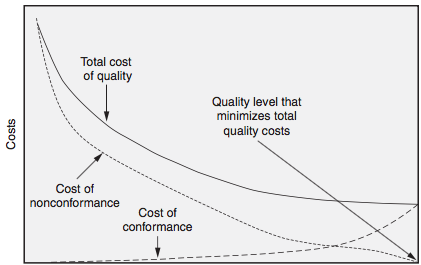
\includegraphics[width=90mm]{imagenes/CurvaCostesCalidadFin.png}
	\caption{Curva de Costes de Calidad al final del desarrollo}
	\label{fig:CurvaCostesdeCalidadFin}
\end{figure}

Una técnica para desarrollar estrategias es la planificación \textit{hoshin}. Desarrollar 4 visiones de lo que debería ser la compañía en 5 años.

Expected Profit = $\sum$ Profit x Probability

Cuando un sistema trabaja por debajo de su nivel óptimo es \textit{suboptimization}.

\subsection{Conductores de la organización y métrica}
Factores clave: hay que sacar datos e información de clientes, productos, servicios, operaciones, mercado, competitividad, proveedores, sindicatos, costes, gobiernos y cumplimiento del rendimiento. Indicadores.

\textbf{Voice of the Customer (VoC)}: factor clave el cliente y el conocimiento del mercado. Las relaciones con clientes y la habilidad de determinar cómo adquirir un nuevo cliente, satisfascerlo, conseguir su lealtad para retenerlo y expandir el mercado. VoC es el proceso para capturar información relacionada con los clientes. La intención es anticiparse a los requerimientos de cliente, necesidades y deseos. La meta es conseguir la lealtad para construir relaciones entre-con clientes. VoC puede incluir reunir e integrar datos de encuestas, datos de la web, datos de garantías, registros de quejas y toda aquella información que afecta a la compra y a las decisiones que toma un cliente.

\textbf{Balanced Scorecard (BS)} (tarjetas de puntuación): miden desde rezagadas hasta líderes las areas: financieras, cliente, procesos internos, y carrera del empleado. Las medidas rezagadas son aquellas al final del evento y las lideres son las que ayudan a conseguir objetivos y se miden antes del evento. 

Este método sirve para saber que es lo que tienen que medir las compañías en orden de equilibrar los resultados financieros. 
BS no es solo un sistema de medida, también es un sistema de gestión que permite a las organizaciones focusear su visión y estrategia convirtiéndolas en actos. Provee feedback en procesos internos y externos. Una vez completamente integrado, el BS convierte el plan estratégico en el centro nervioso de la empresa.

\textbf{Scoreboard/Dashboard}: representación visual que da una visión rápida de la compañía a tiempo real. Es crítico para ayudar al empleado a predecir ventas, cash flow, beneficio y da claridad a la actuación y dirección de la compañía. Debe ser una herramienta crítica de toma de decisiones usada en las operaciones del día a día. Tres pasos para construir un efectivo \textit{Dashboard}: 1) conocer los promedios y el benchmark de la industria. 2) conocer nuestra posición y trayectoria sobre estos promedios y el benchmarking 3) desarrollar cada llamada al BS en un conjunto comprensivo de la compañía, no solo las partes implicadas.

\textbf{Key Performance/Process Indicator (KPI)} (indicador clave de rendimiento): Medida cuantificable que acordada de ante mano, refleja el éxito de los factores críticos. Hay que saber elegir que medidas necesitas trackear/perseguir en tus proyectos. 

\section{Principios Lean en la organización}

Lean: valor, waste y el proceso de crear valor sin waste. Añadir valor sin reducir nada mas es la idea. Toyota Production System es el origen y la clave del Lean. La casa del TPS es lo suyo. Supongo que mas adelante se verá más claro.

\begin{figure}[ht!]
	\centering
	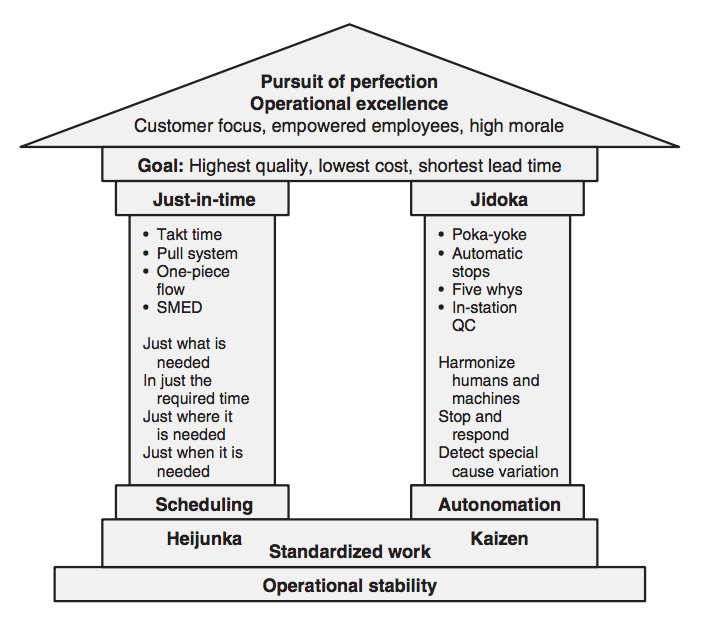
\includegraphics[width=120mm]{imagenes/TPSHouse.png}
	\caption{TPS House}
	\label{fig:TPS House}
\end{figure}

\subsection{Value}

El concepto que mas preocupa a los negocios en los años recientes es \textit{valor}. La percepción de la utilidad y necesidad de un producto o servicio. 

La gente coge coches japoneses por calidad, confianza y eficiencia. La gente coge coches alemanes por otros valores, el orgullo de marca por ejemplo. Los coches americanos son comparables con ambos, pero ellos creen en la lealtad del cliente. 

Un paso tiene valor añadido dentro de un proceso si: el cliente reconoce el valor del producto/servicio, si esto transforma el producto, si está bien hecho a la primera.

Non-value-added, rework, son actividades por las que el cliente no está dispuesto a pagar. El cliente está dispuesto a pagar por la impresión de un documento pero no por las correcciones del proveedor. "question everything" para buscar actividades non-value-added. Siempre hay zonas grises entre valor añadido y no valor añadido. Esto ocurre con inspección y testeo. El cliente no quiere problemas, por lo que inspección es valor añadido, pero la solución es mejorar el proceso hasta el punto de que no tenga que ser inspeccionado. Por otro lado, el sello de la IFS da categoría, así que hacer lo que el sello pida es lo suyo, ya que tenerlo da un valor añadido.

Los 14 principios del Camino Toyota: 1) decisiones de gestión en una filosofía de largo plazo. 2) proceso continuo que lleve los problemas a la superficie. 3) pull system para evitar overproduction 4) nivel de carga de trabajo 5) construir cultura de parar a arreglar problemas para tener calidad desde el primer momento 6) estandarizar tareas y procesos 7) controles visuales 8) tecnología fiable y probada 9) crecer lideres que entienden el trabajo a fondo, viven la filosofia y enseñan a otros 10) desarrolla gente y equipos que sigan la filosofia de la compañia 11) respeta la red de compañeros y proveedores retandolos y ayudandolos a mejorar 12) ve y mira por ti mismo para entender la situacion 13) toma decisiones en concenso y teniendo en cuenta todas las opiniones 14) empieza una organización que aprenda la mejora continua.

\subsection{Herramientas Top Lean}

\textbf{5S (o 6S, o 7S)}. Método de organización del lugar de trabajo para mejorar la eficiencia. El orden: \textit{Sort}: Lo que no hace falta o rara vez hace falta, fuera. Muchas cosas da lugar a desorden y desorden da lugar a pérdida de tiempo. \textit{Set in order}: Colocación de las cosas necesarias en el sitio necesario: instrucciones, herramientas, gafas de seguridad. \textit{Shine}: la limpieza es importante. Una vez resuelto (si es un ejercicio intelectual) hay que dejarlo bien organizado y limpio para que se entienda, esa es la filosofía de la limpieza. \textit{Standarize}: desarrollar checklist, starndarts e instrucciones de trabajo para tener un orden. \textit{Sustain}: mantener las otras 4 S. Las 5S mejoran la productividad y la eficiencia, reduce los accidentes. La gestión debe dar poder a los empleados para que ellos puedan propiedad de sus areas de trabajo. Las otras dos \textit{Safey}-seguridad y \textit{Oversight}-asegurar a la primera.

\begin{figure}[ht!]
	\centering
	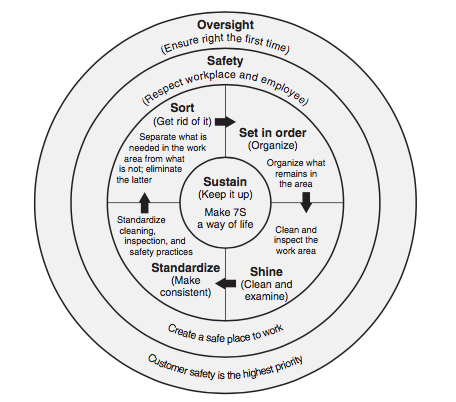
\includegraphics[width=90mm]{imagenes/7S.png}
	\caption{7S adaptation}
	\label{fig:Las7S}
\end{figure}


\textbf{Andon}. Sistema de feedback visual (semáforo) para advertir del nivel de calidad de producto.

\textbf{A3}. Un formato a 3 que contenga: Antecedentes, Situación Actual, Análisis de Causas, Objetivos de Mejora, Acciones de mejora, Plan de acción, Seguimiento de los resultados. No todos los problemas necesitan un A3, solo los complejos y no-evidentes.

\textbf{Gemba}. Ir a planta, allí es donde ocurren las cosas!. Gestión mientras caminas.

\textbf{Heijunka}. Calendario productivo orientado en hacerlo en pequeños bloques de secuencias, en el mismo proceso. Para reducir tiempos muertos y tener bajos niveles de inventario.

\textbf{Hoshin Kanri}. Quality Function Deployment. Consiste en alinear las metas de la compañía (strategy) con los planes a medio plazo (tactics) y las operaciones de trabajo (actions). 

\textbf{Jidoka (Autonomation)}. Por qué hacerlo a mano si una máquina lo puede hacer mejor. Sobre todo si son cosas tediosas. 

\textbf{Kaizen Continuous Improvement vs Kaizen Events}. Mejora continua. \textit{Kaikaku} es un evento Kaizen. Resultados rápidos. Apoyo de la gestión para cada iniciativa. Si los empleados no pueden mejorar el proceso entre 3 - 5 días, la organización necesita reajustar la cultura.

\textbf{Kanban (Pull System)}. El sistema es mejor controlado cuando material e información fluye hacia dentro y fuera de los procesos de manera suave y racional. Ocurre que muchas veces llega antes de tiempo, informacion confusa... Un sistema Kanban da la información necesaria en el momento oportuno. Funciona usando unas visual cards.

\textbf{Overall Equipment Effectiveness (OEE)}. El concepto de medir la efectividad de una operación: \textit{availability, performance and quality}. A * P * Q. 

\textbf{Single Minute Exchange of Die (SMED)}. Rápido y efectivo camino para convertir un proceso operativo en un producto hacia el siguiente. Los grandes cambios son la clave para reducir lotes de producción. \textit{Pensar en esto para Lean Office}.

\textbf{Standar Work}: 9001 es la ley para esto. Poco que decir, crear mapa de procesos, y esas cosas.

\textbf{Takt Time} del aleman \textit{taktzeit}. La batuta de una orquesta. Goles, velocidad, tiempos. Ajustar producción con demanda.

\textbf{Theory of Constraints}. Metodología de problema-solución que busca el enlace más debil de la cadena. Normalmente es el mas lento. Identificar, Explotar (mejorar), Subordinar (el resto a este), Elevar (revisiones, inversiones, mejora del weak) y Repetir.

\subsection{Muda}

El waste (muda) viene de varias fuentes. Cuales?

\textbf{Overproduction}. Hacer mas de lo que necesita el siguiente proceso. Principal síntoma \textit{Work In Process WIP}.

\textbf{Excess motion}. Workplace layout. Ergonomic problems, tiempo gastado buscando o moviendo provisiones o equipo.

\textbf{Waiting}. Esperas, setups largos, gente que no aparece, la gente se demora. 

\textbf{Inventory}. Tienes inventario? el control sobre él es un gasto. Equilibrio control de stock vs ciclo económico, retorno de la inversión.

\textbf{Excess Movement of Material/Transportation}. Los movimientos de handling y storing matan. Un plant layout bien puesto para evitar esto. Function-oriented departments necesita muchos movimientos.

\textbf{Defect Correction}. Corregir defectos. Actividad non-value added. Tipicas causas: mal equipo de mantenimiento, mal sistema de calidad, malas instrucciones de trabajo y mal diseño. 

\textbf{Excess Processing/Overprocessing}. Dificiles de reconoces. Demasiados procesos. 

\subsubsection{Otros}

\textbf{Falta de creatividad}. Empleados tienen que tener ideas para mejorar los procesos.

\textbf{Perfeccion}. Evitar la perfección exacta. 

\subsection{Value Stream Mapping} 

\textit{Value Stream} es una serie de actividades que hace una empresa: pedir, diseñar, producir, entregar productos/servicios. Un value stream empieza por los proveedores de los proveedores y acaba con los clientes de los clientes. Componentes: 1. Flow materials desde proveedor hasta entrega a cliente (los pedidos entran semanalmente en camion, los materiales se mueven hasta la zona de produccion y al almacen de producto terminado, producto terminado se entrega a cliente), 2. Transformation of raw materials (pasos de produccion rollo cortar, moldear, forjar...), 3. El flujo de información requerido para ayudar al flujo de material y a la transformación (ordenes de compra a provedores, ordenes internas de trabajo, shipping notice...).

Value Stream Map usa gráficos con iconos simples para ilustrar el movimiento del material, inventario, work-in-progress, operadores... Un Value Stream Analysis es el que descubre \textit{wastes} ocultos en la organización. Aplicar Lean Thinking para dividir un \textit{path} en diferentes pasos: 1. Producir un \textit{value stream map (value chain diagram)}. 2. Analizar las notas de inventario pensando en reducirlo o eliminarlo (inventario = coste del espacio, perdida de calidad, V2 v3 v4..., el dinero se puede invertir en otras cosas), 3. Analizar los non-value steps para eliminarlos, 4. Determinar como es conducido el flujo (p.e.: en funcion de pedidos del cliente), 5. Extender el value stream map hasta los proveedores (compatibilidad entre sistemas-codigos de barras).

\begin{figure}[ht!]
	\centering
	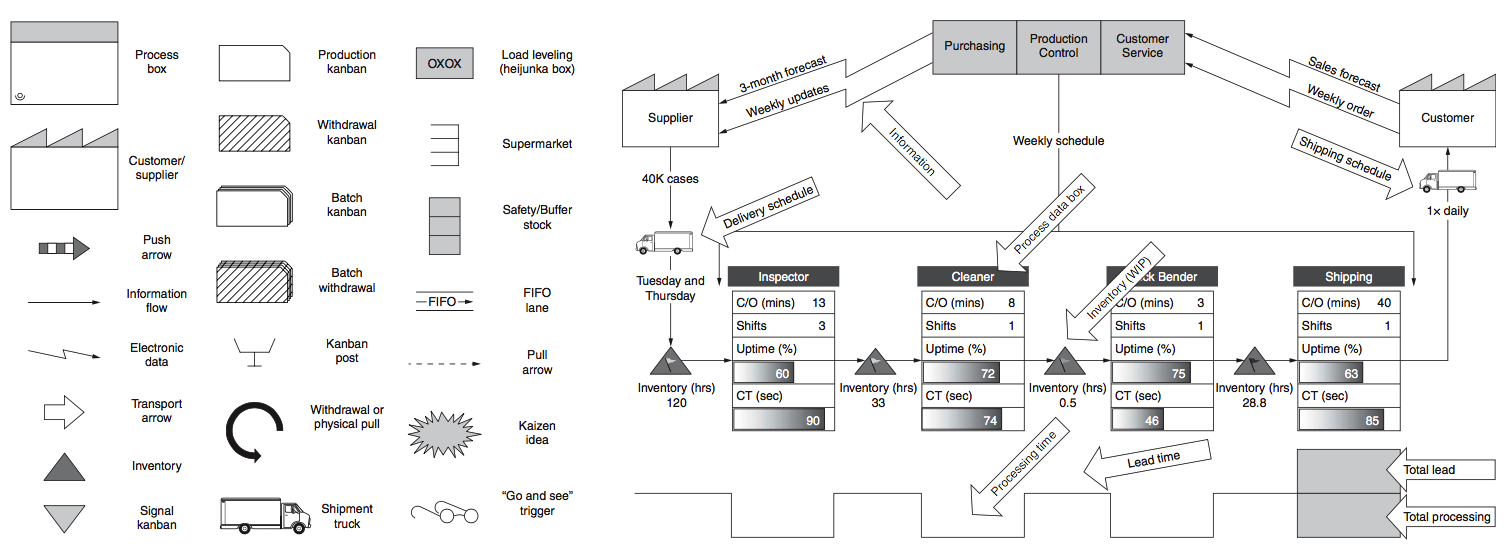
\includegraphics[width=170mm]{imagenes/ValueStreamMapping.png}
	\caption{Value Stream Mapping}
	\label{fig:ValueStreamMapping}
\end{figure}

\section{Diseño para metodologías Six Sigma (DFSS)}

DFSS se apoya proceso estratégico de negocio/ingenieria y en procesos capaces de reducir y gestionar variaciones: con DMADV (define, measure, analyze, design, verify) y con IDOV (identify, design, optimice, verify). Hay batiburrillo de sigmas DFSS, DCOV, ICOV, DMEDI, IDDOV, GD. Se use el que se use, pero hay que recordar: robustez del sistema usado, no abrir mil proyectos, uno para cada síntoma, evitar perder el tiempo alimentando el sistema de datos y ratings, alcance vago o pequeño. Lo que no puedes controlar se llama \textit{noise}. \textit{noise strategy} para mejorar el proceso.

Usamos DFSS para aumentar la satisfacción de cliente, reducir variaciones, tener un diseño robusto, bajar costes de garantía, mejorar durabilidad, incrementar facturación-ganancias y producción (ésta última a través de bajar downtimes por defectos).

\subsection{IDOV} \textit{Identify} \textit{Design} \textit{Optimize} \textit{Verify} similar al MAIC del Six Sigma (\textit{measure, analyze, improve, control}).

\textit{Identify Phase}: identificar requisitos de producto y cliente, establecer caso de negocio, identificar aspectos técnicos, critical to quality (CTQ) variables, y limites de especificaciones, roles y responsabilidades, hitos.

\textit{Design Phase}: Formular el concepto, identificar posibles riesgos usando FMEA (failure mode and effects analysis), para cada detalle técnico, identificar parámetros diseño, usar DOE (design of experiments) y otras herramientas de analisis para determinar CTQs y su influencia en los requisitos técnicos.

\textit{Optimize Phase}: Evaluar las posibilidades del proceso y llegar a conocer bien los limites CTQ. Optimizar el diseño minimizando los CTQs, prueba-error, estadisticas y tolernancias.

\textit{Validate Phase}: Prototipado, evaluar actuacion, fallos, confianza y riesgo, design iteration y revisión final de producto.

\subsection{DMADV} Para cuando el producto no existe y ha de ser desarrollado. O ya existe pero no se conocen las necesidades del negocio o del cliente. 

\textit{Define}: Targeting prioridades.

\textit{Measure}: combinación de análisis técnico y competitivo del producto. 

\textit{Analyze}: Aproximaciones de estadística e investigación, para establecer prioridades y confianza.

\textit{Design}: Design for/to Cost: busqueda de alternativas en procesos, materiales, métodos... Design for Manofacturing/productibility/assembly: pequeños cambios que hacen que sea mucho mas barato fabricarlo. Design for test: donde testing es critico, lo mejor es hacer test tempranos en el ciclo de producción. Design for maintability:si necesitas muchos downtimes y reparaciones. Design for Robustness: test en todos los ciclos de vida, y partes, ensamblajes y sub. Design for usability: VALIDATION!  puede ser medido y mejorado. Extended for functionality: otras features desde el pto de vista del diseño. Design for efficiency: consumo minimo de recursos. Design for Performance: la mejora de los microchips es un ejemplo. Design for security: preserva la integridad del producto. Design for scalability: 

\textit{Verify}: Es necesario asegurar los resultados del diseño de los objetivos. 

\subsection{FMEA} Usa FMEA para evaluar el proceso o el producto y determinar que causa el fallo y los efectos que pueden tener. 
Identifica y usa escala, calcula el Risk Priority Number (RPN) y analiza los resultados.

La esencia del \textit{failure mode and effects analysis} es el estudio del riesgo. Riesgo es lo incierto de un evento. Riesgo es la posible influencia buena o mala de un producto en un entorno. El riesgo se puede definir como impact (severity)  probability (ocurrence) y event (detection). Segun Risk Road Map ISO 31000:2009: gestión del Plan risk / herramientas del risk identification / analizar y evaluar riesgos / plan risk response / monitor y control del risk.

\begin{figure}[ht!]
	\centering
	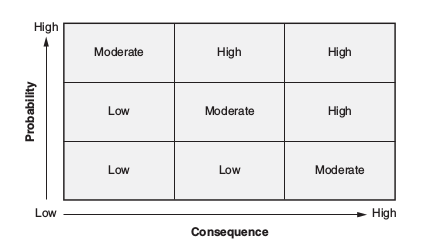
\includegraphics[width=90mm]{imagenes/RiskMatrix.png}
	\caption{Risk Matrix en FMEA PRN}
	\label{kMatrix}
\end{figure}

FMEA es una herramienta front-end. Un producto/proceso de éxito requiere anticiparse a los problemas y para ello hace falta tener jerarquizados cuales atacar antes, y/ como atacarlos. \textbf{Mirar Effective FMEAS}. El documento de gestión FMEA se tiene que ir controlando por versiones, incluyendo y quitando cosas, ya que es un documento vivo. Beneficios del FMEA: evaluación a todos los clientes (internos y externos), ayuda en la evaluación de requerimientos y alternativas, ayuda a centrarse en donde pueden aparecer los problemas criticos y como paliarlos/evitarlos/controlarlos, desarrollo de una lista de actuaciones priorizada, ayuda para evaluar el propósito del proceso.

\begin{figure}[ht!]
	\centering
	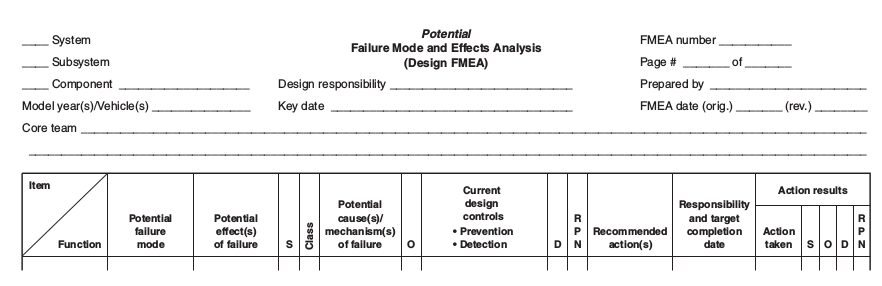
\includegraphics[width=170mm]{imagenes/PlantillaFMEA.png}
	\caption{Cabecera de una plantilla FMEA}
	\label{fig:PlantillaFMEA}
\end{figure}

\begin{figure}[ht!]
	\centering
	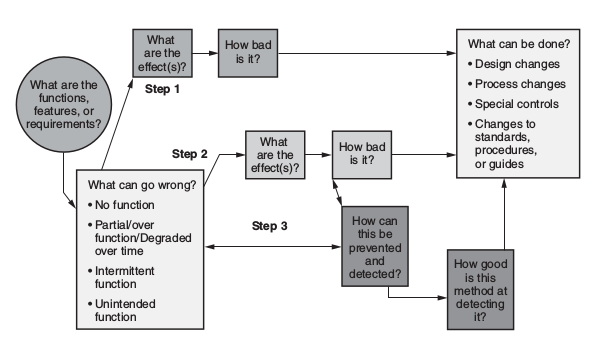
\includegraphics[width=90mm]{imagenes/FMEAFlowchart.png}
	\caption{Diagrama de flujo de FMEA}
	\label{fig:FMAFlowchart}
\end{figure}

Pasos del FMEA: 1. Lista los pasos claves de un proceso 2. brainstorm de porque puede fallar cada paso 3. lista de efectos de los fallos 4. ranking de severidad para los efectos 5. causa y frecuencia de los fallos 6. controles para la detección 7. calcular RPN 8. Ordenar por críticos los RPN. 9. Desarrollar plan de accion, asignando persona-responsabilidad 10. Re-Calcular el RPN una vez implantado.

\subsection{Do's} 1. Da formacion de FMEA antes de asignar equipos 2. Enfoque de equipo 3. Pregunta a expertos si es necesario 4. Habla con el cliente de como va a utilizar el producto 5. brainstorm de los posibles fallos. 6. Si dos riesgos tienen la misma RPN, se queda encima el que tenga mas severidad. 7. completa la accion y reasigna la severidad. 8.Actualiza el FMEA con los nuevos riesgos aprendidos.

\subsection{Don'ts} 1. No copies el S-O-D de una industria a otra. 2. Intenta no usar una escala de 1-10, de 1-5 mejor. 3. No hagas escalas especializadas sino es completamente necesario. 4.	No manipules los datos.

\begin{figure}[ht!]
	\centering
	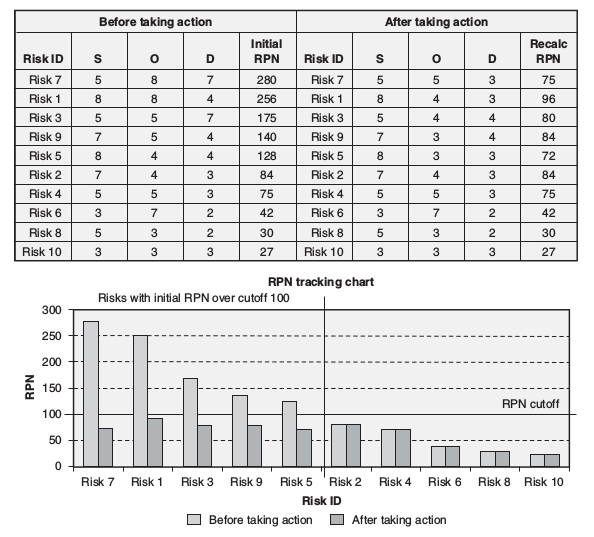
\includegraphics[width=140mm]{imagenes/FMEAPrePos.png}
	\caption{Report final de un FMEA}
	\label{fig:FMEAPrePos}
\end{figure}

\part*{Definicion}

Preguntas críticas de la fase de definición: donde estamos? cual es el problema? donde queremos estar? como vamos a llegar allí? como sabremos que hemos llegado a ese punto?

Antes de empezar, comprobar que la gestión y la economía del proyecto están alineadas. Mas tiempo frente a una buena planificación, mayor será el éxito. 

\section{Identificación del proyecto}
\subsection{Project Selection}

Describir el proceso de seleccion de proyecto y que factores deben ser incluidos para considurar si usar DMAIC u otro tipo de problem-solving process. Lo suyo es que haya un departamento o comité para decidir qué proyectos se pueden llevar a cabo y cuales no, ya que todas las ideas a la vez son imposibles. Cada propuesta debe tener medidas sobre el problema que plantean resolver y el impacto de éstas sobre la organización. Managers suelen coger la que ahorre más dinero a la compañía.
Proyectos que tengan que ver con el análisis de datos, para el equipo de Six Sigma. Los que tengan que ver con mejora de procesos, con el equipo de Lean Manufacturing.

\subsection{Process Elements}

Definir y describir los componentes del proceso	y límites (boundaries). Reconocer como los procesos cruzan varias areas funcionales y los retos que resultan de los esfuerzos de mejora de procesos. Los procesos se pueden subdividir en subprocesos.
Por ejemplo, el proceso de payroll tiene subprocesos: reunir la información del reloj de fichar, hacer deducciones, ...

Para definir bien un proceso hay que marcar donde empieza y donde acaba. Los límites (boundaries). Los procesos transversales pueden tener subprocesos límite, definidos por la estructura del negocio, geografía...

\subsection{Benchmarking}

Entender que hay varios tipos de benchmarking, incluyendo la competitividad, la colaboración y las buenas prácticas.
Pueden ser internas, contra otros procesos internos o externas. Las fuentes de información del Benchmarking vienen de publicaciones, reuniones profesionales, investigaciones universitarias, feedback de clientes, visitas, análisis de productos de competidores...

Operaciones de Benchmarking: analizar la operativa, conocer los líderes del mercado, incorporar lo mejor de lo mejor, ganar superioridad. 

Internal benchmarking: facil acceso a otros dptos. sin embargo, el límite de mejora está reducido al estilo de la compañía.

Competitive benchmarking: fuerza a la compañía a tener una perspectiva externa. Sin embargo, fijarse en las prácticas de las industrias puede limitar el alcance de altos niveles de actuación.

Funcional benchmarking: comparas funciones similares, normalmente se busca fuera de la empresa y permite conseguir más partners de benchmarking.

Collaborative benchmarking: cooperación entre varias organizaciones para lograr resultados de benchmarking. Esta práctica permite el acceso a benchmarking partners  mas especificos.  

\subsection{Inputs y outputs de procesos}

Identificar las variables del input y las del output y evaluar sus relaciones usando Supplier, Inputs, Process, Output, Customer (SIPOC model).

Es clave definir los límites del proyecto, por motivos como este fracasa.

Dividir los procesos por functional areas (dptos) y organizations (suppliers, intercompany, teammate company, ...), esto se puede identificar con diagrama SIPOC y con un flowchart estilo swim-lane y un mapa de procesos podemos reconocer las interacciones entre ellos. Retos que te encuentras cuando defines esto: quien es el dueño del proceso, quienes comparten información, medidas (en que mides? camiones/horas, euros/día), conocimiento del proceso (supply chain no sabe como funciona manufacturing).

Si los retos tienen riesgos potenciales asociados, habría que asociar actividades para minimizarlos.

\subsubsection{Systems Thinking}

La identificación y consideración de todos los diferentes elementos individuales que interaccionan con un propósito común a hacia una gran función se considera \textit{System Thinking}. ST es sobre usar herramientas y me todos disponibles para saber que se está haciendo en una operación específica y como esa actividad afecta tareas y productos posteriores y como priorizar tareas.

ST sirve para entender mejor los procesos y como influyen los parámetros. Ejemplo: proveedor envia X producto con algo mas de humedad de la cuenta, como hay que modificar el proceso para que se ajuste. 

\subsection{Dueños y Stakeholders}

Identifica los dueños de los procesos y los diferentes grupos de interés (stakeholders) en un proyecto.
Los dueños de los procesos son los que tienen la responsabilidad de ejecutar e implementar procesos específicos. Los mejores métodos para mejorar los procesos usan equipos de dueños y de todos los stakeholders ya que éstos últimos tienen mejor conocimiento sobre el proceso, sobre las ideas para mejorar, se preocupan por las consecuencias del cambio en un proceso. Por lo tanto stakeholders en un proceso son: operadores, managers, clientes, proveedores, ...

\section{Voice of the Customer (VOC)}

\subsection{Identificar al customer}
Customers puede haber de dos tipos: internos, que trabajan en el proceso, externos. Pasa identificar customers: brainstorming, SIPOC, analisis de márketing, trackear un producto hasta la entrega.

Al igual, se pueden dividir los customers por grupos: Internos/Externos, por edad, por localización, clima, lengua, por industria.

\subsection{Datos del customer}

Hace falta conseguir datos: encuestas, observar grupos, entrevistas, ... Identificar los elementos clave para hacer efectivas estas herramientas. Revisar colecciones de datos para eliminar indeterminaciones.
¿Como saber lo que el cliente quiere? preguntándole. El cliente es experto en lo que hace, sabrá lo que necesita. 

El foco para un GB es, internamente, hablar con la gente para saber qué hacen y cómo podríamos hacer que fuera más fácil hacerlo: lo que quiere, requisitos y expectativas. 

Para capturar datos del customer podemos utilizar: VoC, surveys, QFD (Quality function deployment), entrevistas, Focus groups!

Lo suyo es seleccionar aleatoriamente un gran grupo de clientes y aplicar un método de manera estadísticamente válido. La info debe ser objetiva, con precisión y consistencia, evitando la ambigüedad. 

\subsection{Requisitos del cliente}

Usamos QFD (Quality Functions Deployment) para traducir los requisitos del cliente en características del producto y oportunidades de mejora. Una de las aplicaciones mas importantes de Six Sigma es diseñar y rediseñar procesos y productos, para conseguir el menor coste posible.

QFD (o \textit{House of Quality}) tiene de input VOC. La matriz QFD muestra el enlace entre VOC y los requisitos técnicos resultantes.

\begin{figure}[ht!]
	\centering
	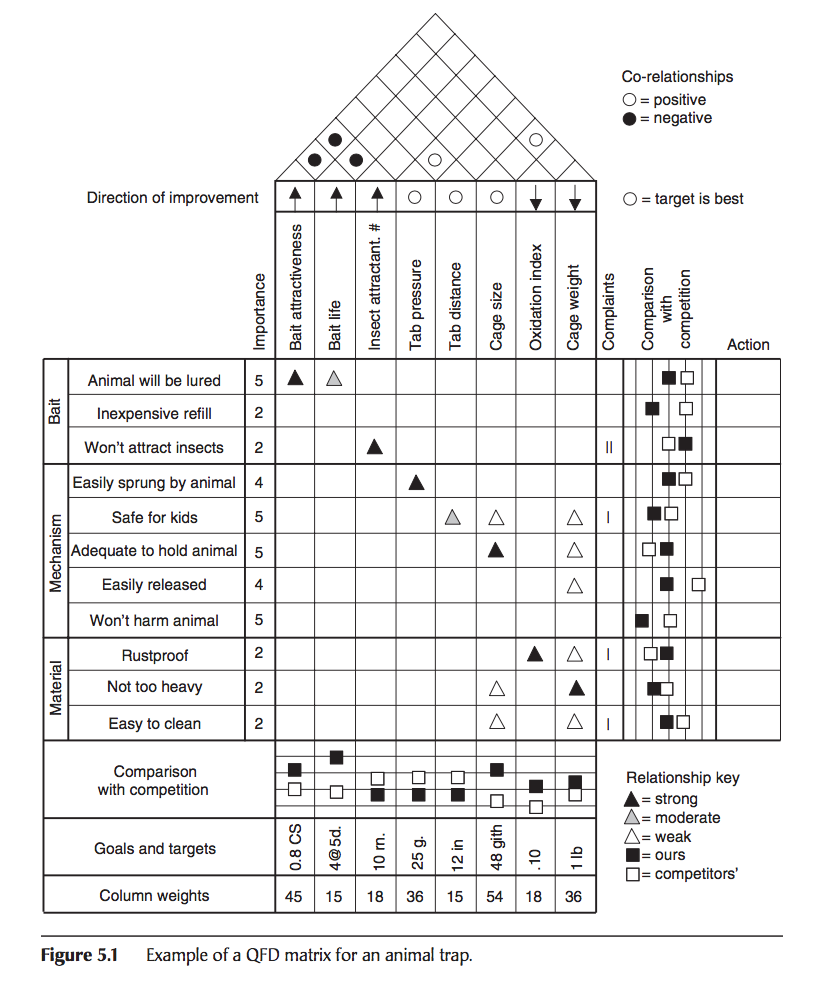
\includegraphics[width=150mm]{imagenes/ExampleQFD.png}
	\caption{Ejemplo de un QFD}
	\label{fig:ExampleQFD}
\end{figure}

QFD puede ser aplicado para mejorar calidad. En la matriz, los What's, se traducen por \textit{must have} o por \textit{expected to have}. QFD ayuda a la calidad de cliente conducida.

\section{Project Management Basics}

\subsection{Project Charter}

Describir y definir elementos de un Project Charter, desarrollar el problema que incluya datos base o el estado actual para ser mejorado y las metas del proyecto.

Un \textit{charter} es un documento de declaración con el propósito del proyecto.
Permite tener a los equipos de desarrollo alineados con la dirección de la empresa. Debe incluir: 

\begin{itemize}
	\item Problem statement. Qué necesita ser mejorado.
	\item Purpose. Establece metas y objetivos del proyecto.
	\item Benefits. Por qué irá mejor la empresa cuando se consiga el objetivo.
	\item Scope. Limitaciones: tiempo, presupuesto, recursos, ..
	\item Results. Define el criterio y métricas para el éxito del proyecto.
\end{itemize}

\textit{Project Planning} Nos acerca a la monitorización del como y cuándo un proyecto será llevado a cabo. Necesario: información de los procesos, comunicación, negociación de recursos, incremental y modular planificacion, asegurar hitos medibles y facilitating top management involvement.

\subsection{Project Scope}

Usando SIPOC, brainstorming, diagrama de pareto, podemos definir y documentar el alcance del proyecto. Normalmente el alcance está basado en el \textit{Problem Statement}.

\subsection{Project Metrics}

Una planificación de proyecto sin la actuación de medición es poco menos que un papel absurdo. La medición clave (key metric) enlazan directamente las mediciones con las metas. Si vamos en contra del tiempo: \textit{Percentage of work accomplished on time}, \textit{Percentage of work accomplished on budget}, \textit{disponibilidad de recursos}...

KPI (Key process indicators) es un valor medible que demuestra la efectividad de una compañía consiguiendo sus objetivos claves de negocio.

\subsection{Project Planning Tools}

Gannt, CPM (Critical Path Method), PERT para planificar proyectos.
Las herramientas difieren según el tamaño y alcance del proyecto. La documentación se mantiene viva durante el desarrollo de todo el proyecto.

\subsection{Project Documentation}

Metas y objetivos. Sponsors y accionistas. Planificación y calendario. Hitos. Presupuesto. Límites. Roles y responsabilidades. Métricas para evaluar el proyecto.

Además del \textit{Project Charter} y el \textit{Project Management Plan} planes adicionales pueden ser utilizados para cada actividad.

\subsection{Project Risk Analysis}

El análisis de riesgo de un proyecto se incluye durante la fase de planificación. Identificar riesgos, asociar impacto y posibles planes para minimizar el riesgo. El análisis de riesgo hay que revisarlo y actualizarlo utilizando SWOT (strengths-weaknesses-opportunities-threats), RPN, FMEA, formula for expected profit.
Un buen análisis de riesgos necesita de que las grupos apropiados estén presentes.

Aspectos de riesgo a considerar incluyen el impacto potencial en: conocer las metas establecidas, el calendario planificado, fuentes identificadas, seguridad, productividad, servicio, confiabilidad, conocer los requerimientos y expectativas del cliente.

\begin{figure}[ht!]
	\centering
	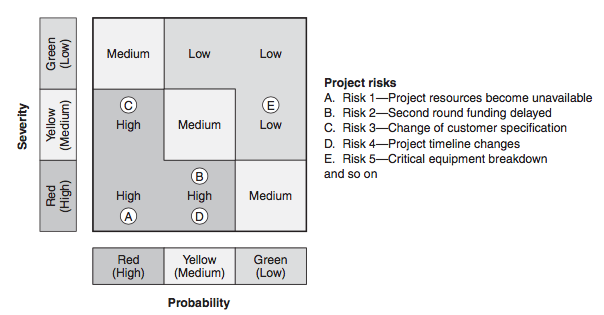
\includegraphics[width=90mm]{imagenes/RiskMatrix2.png}
	\caption{Matriz de riesgo}
	\label{fig:RiskMatrix2}
\end{figure}

A través de cosas que ya han pasado antes, riesgos, brainstorming se determinan los Project Risks. Después de identificarlos, minimizarlos y verificar las actuaciones que los pueden desencadenar son cosas que tienen que estar en el ciclo de vida del proyecto. 

Si un riesgo existente es: proveedor clave que no entrega a tiempo, la mitigation activity es buscar un nuevo proveedor.
Si un riesgo existente es: un cajero automático, la mitigation activity es: codigo de 6-10 cifras, bloqueo a los 3 intentos.

\subsection{Project Closure}

Revisar con los miembros y sponsors los objetivos logrados con el proyecto, asegurar que la documentación está completa y guardada apropiadamente. Identificaar lecciones aprendidas e informar a otras partes de la organización sobre oportunidades de mejora.

Project Closure no es negociacion, es un paso final para conocer que metas y objetivos se cumplen, que la documentación está OK, y hacer una reunión para cerrar.

Project charter es una excelente herramienta para medir el progreso de un proyecto, con su alcance, metas, objetivos y una cronología.

\section{Management and Planning Tools}

\subsection{Activity Network Diagram}
Es como el PERT, muestra dependencias entre tareas y caminos (en serie o en paralelo). Al igual que PERT o Critical Path Analysis, provee una visión global con nivel de detalle adecuado a la necesidad del proyecto.

\begin{figure}[ht!]
	\centering
	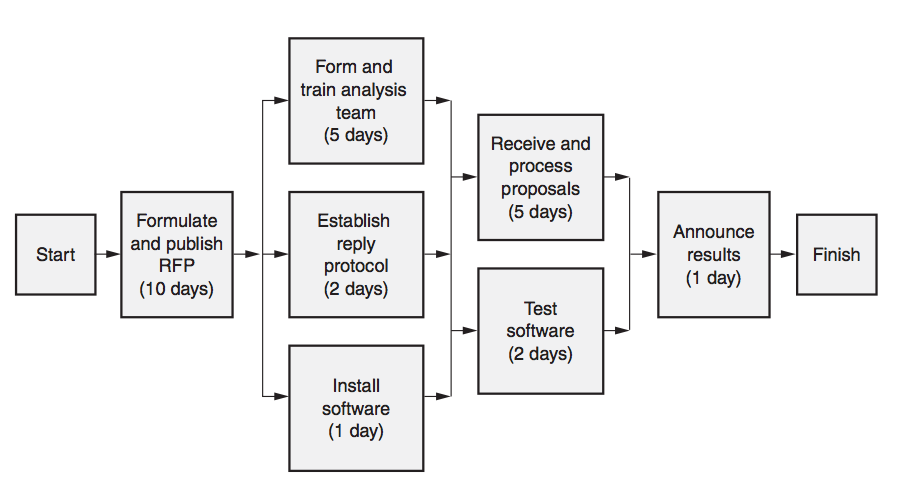
\includegraphics[width=120mm]{imagenes/AND.png}
	\caption{Activity Network Diagram}
	\label{fig:ANDDiagram}
\end{figure}

\subsection{Advanced Quality Planning} 

Se basa en la idea de que las planificaciones solidas previenen sorpresas y salvan recursos útiles de ser malgastados. AQP es un proceso donde primero miramos los parámetros de que vamos a hacer. ¿tenemos suficiente material disponible? ¿tenemos la gente necesaria para hacer el trabajo?¿tenemos las herramientas necesarias para el trabajo? También se llama APQP. 
Es el priemr paso del PDSA (Plan Do Study Act). Esto ayuda a que todos los inputs tengan el output deseado.

\subsection{Affinity Diagram}

Son usados para producri muchas respuestas a preguntas abiertas. ¿cuales son las maneras de reducir ciclo al proceso? Luego intentar asociar entre sí, en diferentes grandes grupos, dichas respuestas. Luego le damos nombre a la agrupación.

\begin{figure}[ht!]
	\centering
	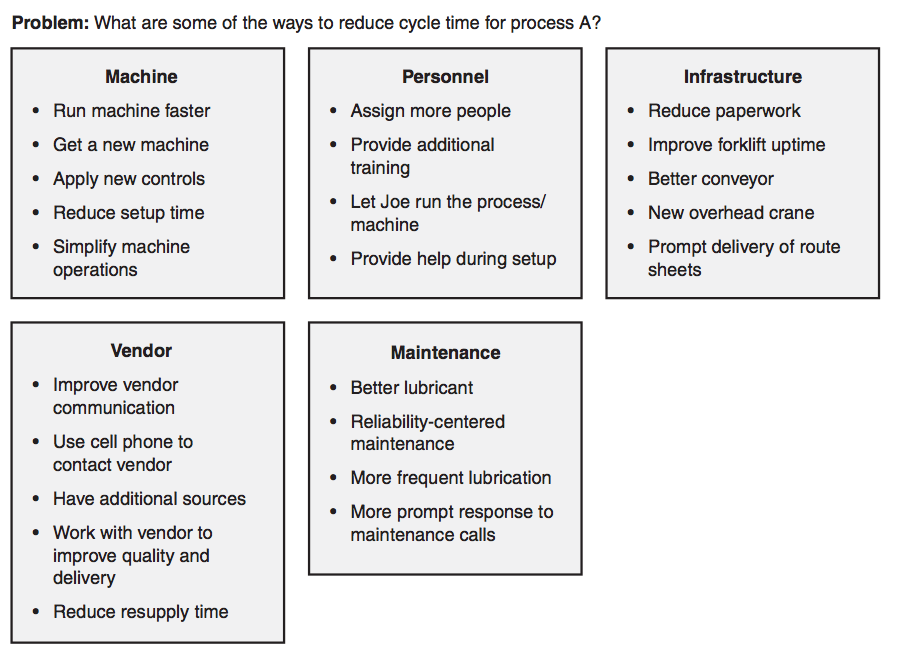
\includegraphics[width=120mm]{imagenes/AffinityDiagram.png}
	\caption{Affinity Diagram}
	\label{fig:AffinityDiagram}
\end{figure}

\subsection{Auditing}

Evaluación de procesos o proyectos contra planes y metas. Esta comprobación de auditoría de calidad es comúnmente establecida en organizaciones a través de sistemas de gestión de la calidad (AS9001, ISO 9001, ISO/TS 16949).

\textit{Audit planning}: preparación para el que va a er auditado, un calendario de auditoria y una notificación de auditoría.

\textit{Audit performance}: evidencias, observaciones, entrevistas.

\textit{Audit report}: resumen con el alcance, actividades, resultados, findings (acciones correctivas), oportunidades de mejora.

\textit{Audit closure}: actividades de seguimiento para asegurar que los planes en accion son implementados de manera efectiva.

Tipos: first-party, second-party, third-party, internal (mas usada en Six Sigma) y external.

Habitualmente están basadas en productos, sistemas, proveedores, cumplimiento normativo.

Be pleasant, you are not a cop. Be prepared. Be factual in what you observe, hiding things doesn't help to improve. Ask questions for clarity. Record your observations. Deja que te guie el auditor interno.

\subsection{Benchmarking}

Consiste en mirar un sistema y aplicar los conceptos de ese, sobre otro. La idea es hacer un win/win entre organizaciones. Pasos básicos: Flowchart del proceso actual. Identificar areas de mejora. Ideas brainstorm. Investigar como otros hacen el proceso. Desarrollar planes de aplicación de ideas. Prueba piloto. Iniciar el nuevo proceso. Evaluar el nuevo proceso.

\subsection{FishBone Ishikawa}

Muestra factores envueltos en una situación. Crearlo a partir del 5W's (What, Why, When, Where, Who), 1H (How) y 6M's (Man, Machine, Methods, Materials, Measurement, Mother Nature, Money, Management).

\begin{figure}[ht!]
	\centering
	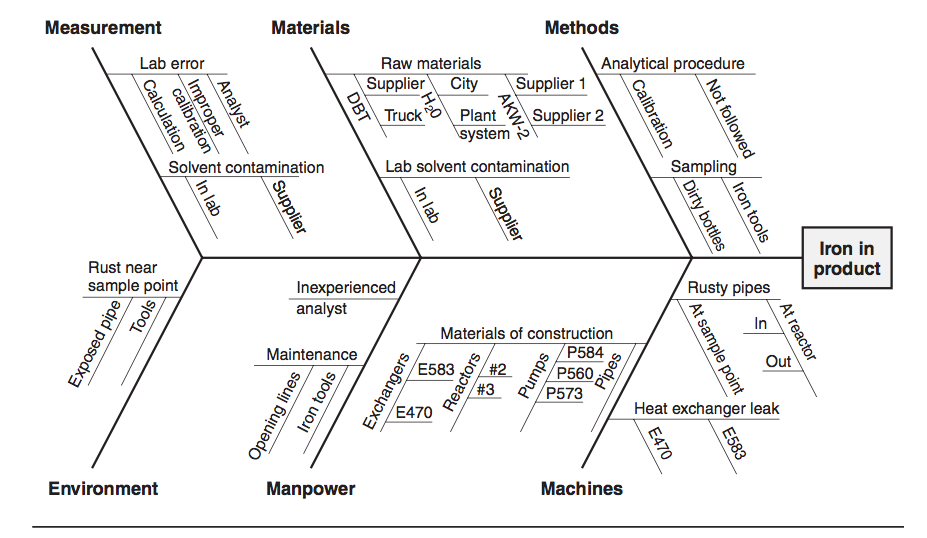
\includegraphics[width=120mm]{imagenes/FishBone.png}
	\caption{FishBone}
	\label{fig:FishBone}
\end{figure}

\subsection{Check Sheets}

Usadas para observar o revisar un proceso, durante su ejecución. Pasos básicos en hacer un check sheet: Identificar y agregar las causas o condiciones que han de ser recogidas. Decidir quien recoge la información, sobre cuantos periodos, y de que manera se recoge. Crear un check sheet que trabajará en la operación donde será usada. Recoger datos como diseños para asegurar consistencia y precisión de la información.

\begin{figure}[ht!]
	\centering
	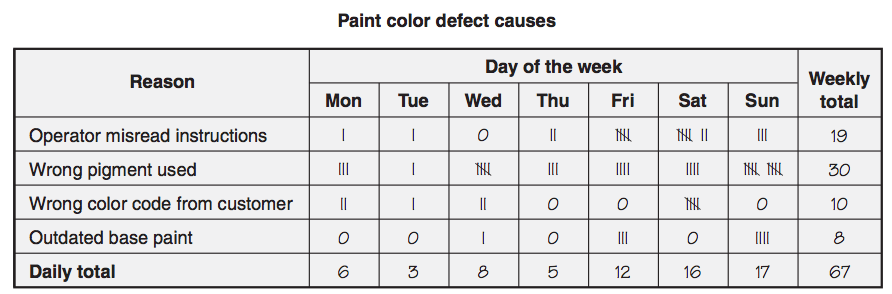
\includegraphics[width=120mm]{imagenes/CheckSheet.png}
	\caption{CheckSheet}
	\label{fig:CheckSheet}
\end{figure}

\subsection{Customer Feedback}

Encuestas, info vía emails, entrevistas dirigidas. Importante conseguir muestras representativas

\subsection{Flowchart}

\begin{figure}[ht!]
	\centering
	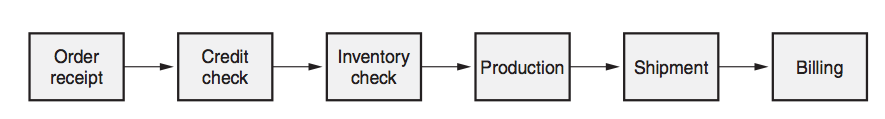
\includegraphics[width=120mm]{imagenes/Flowchart.png}
	\caption{Flowchart}
	\label{fig:Flowchart}
\end{figure}

Pasos: definir el proceso que va a ser diagramado. Decidir los límites del proceso. Averiguar cuales son las actividades que se dan lugar en él. Ordenar las actividades en su secuencia. Flechear los pasos. Que revise el flowchart toda la organización.

\subsection{Focus Groups}

Identificar las metas de la sesión. Desarrollar productos actuales o prototipo. Determinar como las sesiones deben ser conducidas (brainstorming, survey, cause-and-effect, question-response).

\begin{figure}[ht!]
	\centering
	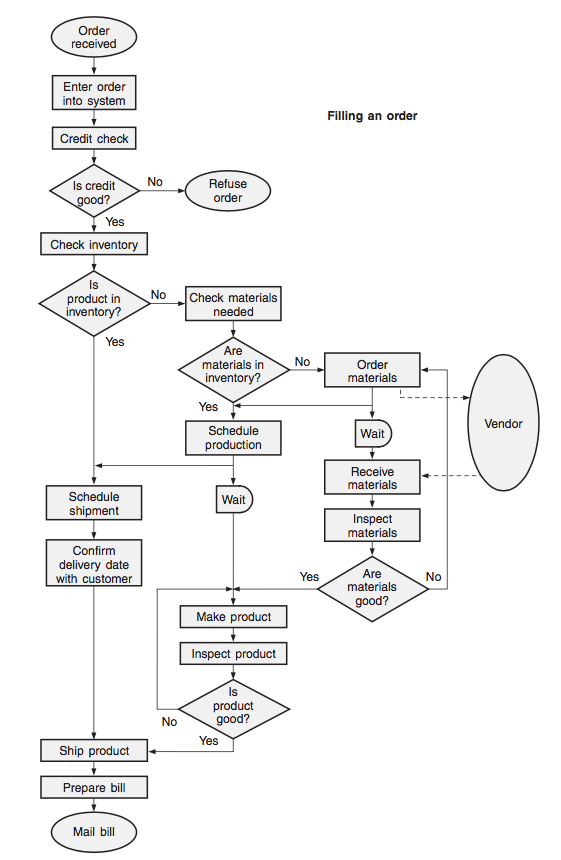
\includegraphics[width=120mm]{imagenes/DetailedFlowchart.png}
	\caption{Detailed Flowchart}
	\label{fig:DetailedFlowchart}
\end{figure}

\subsection{Force-Field Analysis}

Se pone un \textit{Future State} y se hacen dos columnas: Driving forces y Restraining forces. Cosas que suman/restan para conseguir el ojbetivo. A través del NTG (Nominal Group Technique) se hace un ranking con ellas. Y entonces se ve como proceder.

\subsection{Gantt Chart}

Gantt provee de un vistazo rapido las actividades planificadas y el calendario, permitiendo evaluar los recursos claves contra el plan, y también permite la evaluación de la actuación del proyecto frente al plan.

\subsection{Graphical, control and statistical tools}

\subsubsection{Variables Charts}

\begin{itemize}
	\item Averages and range chart.
	\item X and s chart.
	\item IX-MR, XmR, moving range chart.
	\item MA-MR chart.
	\item Target charts, deviation chart, nominal chart.
	\item CUSUM (cumulative sum chart)
	\item EWMA (weighted moving average chart)
	\item Hotelling T2
\end{itemize}

\subsubsection{Attributes Charts}

\begin{itemize}
	\item p-chart (proportion chart)
	\item np-chart
	\item c-chart (count chart)
	\item u-chart
	\item D-chart (total weighted deficiencies)
	\item U-chart 8average weighted deficientes per unit)
\end{itemize}

\subsubsection{Other Kinds of Data}

\begin{itemize}
	\item Short-run charts (Z-charts)
	\item Group charts (multiple characteristic charts)
	\item Paynter charts
\end{itemize}

\subsection{Interrelationship Diagram (DIGRAPH)}

Sirve para identificar relaciones causa-efecto. Normalmente se empieza listando media docena/o una docena entera de preocupaciones, se ordenan y mediante flechas se dirige cual es mas importante que la anterior. Si no se dibuja flecha, es que no tiene importancia sobre otras.

Compara una a una, contra todas las que tiene relación. 

\begin{figure}[ht!]
	\centering
	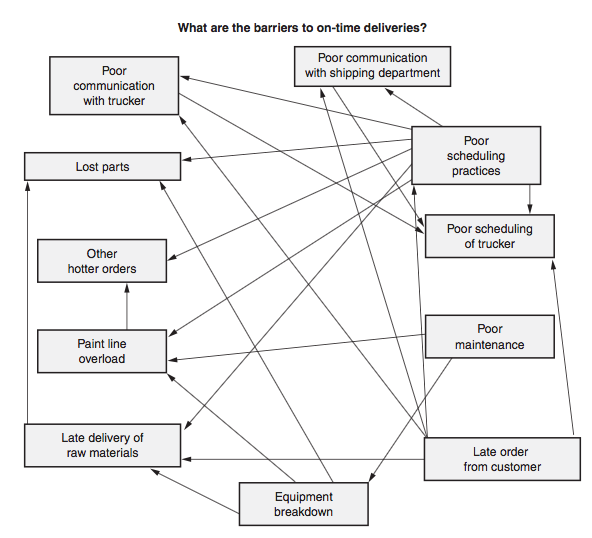
\includegraphics[width=120mm]{imagenes/interrelationshipdiagram.png}
	\caption{Interrelationship Diagram}
	\label{fig:interrelationshipdiagram}
\end{figure}

\subsection{Matrix Diagram}

Para descubrir relaciones entre dos grupos de items. 

\begin{figure}[ht!]
	\centering
	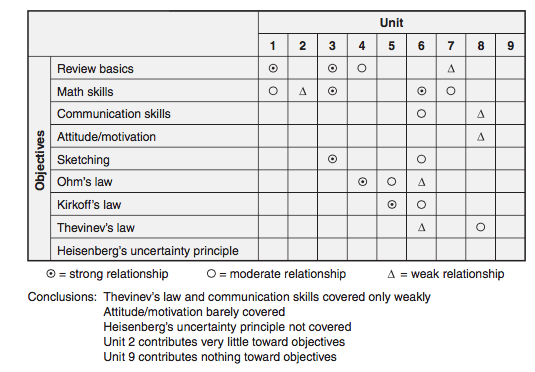
\includegraphics[width=120mm]{imagenes/MatrixDiagram.png}
	\caption{Matrix Diagram de un libro de texto}
	\label{fig:MatrixDiagram}
\end{figure}

\subsection{Nominal Group Technique}

Es un brainstorming con una interacción limitada por grupos. Esto es para que no haya gente que diga mucho y otros no digan nada. El facilitator explica las reglas, el team leader presenta el topic y el equipo tienen como 10-15 minutos para sentarse, pensar y generar ideas.

No se permiten interacciones verbales, las ideas son recolectadas y puestas en un sitio donde todos puedan verlas. Los miembros deben leer las ideas en alto, una a una. A los miembros se les permite expandir las ideas, darles claridad, eliminar redundancia. El team leader debe recoger las ideas y ponerlas en el board, y mantener el anonimato de los contribuyentes.

\subsection{PDCA, PDSA y SDCA}

Plan Do Check Act. Study. Standarize.

\subsection{Priorization Matrix}

Es una ayuda para decidir entre diferentes opciones. Para conseguir el criterio adecuado, se ponen los atributos de cada una de las opciones y se ponderan.

\begin{figure}[ht!]
	\centering
	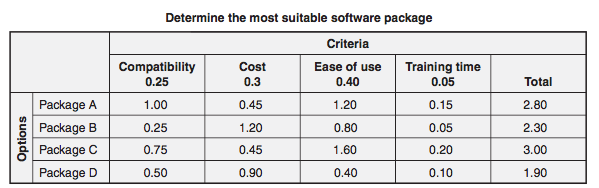
\includegraphics[width=120mm]{imagenes/Prioritizationmatrixexample.png}
	\caption{Prioritization matrix example}
	\label{fig:Prioritizationmatrixexample}
\end{figure}

\subsection{Problem Solving}

\textit{Eight Discipline Approach, 8D}. 

\begin{enumerate}
	\item Usa un team approach. Organiza un pequeño grupo, que conozcan proceso y producto. Un campeón designado.
	\item Describe el problema. 5W2H, SIPOC, flowcharts.
	\item Empieza y comprueba las acciones. Define acciones, verifica la efectividad.
	\item Define y comprueba las raíces de la causa. 
	\item Comprueba la acción correctiva. Que no genere otro problema paralelo: FMEEA y control plans.
	\item Empieza acciones correctivas permanentes. Actualizar procesos y procedimientos para incorporar nuevos procesos. Training cuando haga falta.
	\item Para problemas futuros. Modifica los sistemas de gestión y operativos para reducir recurrence, y similar problems.
	\item Agradece al equipo. Mejoras solo ocurren cuando la gente trabaja junta.
\end{enumerate}

\subsection{Process Decision Program Chart, PDPC}

\begin{figure}[ht!]
	\centering
	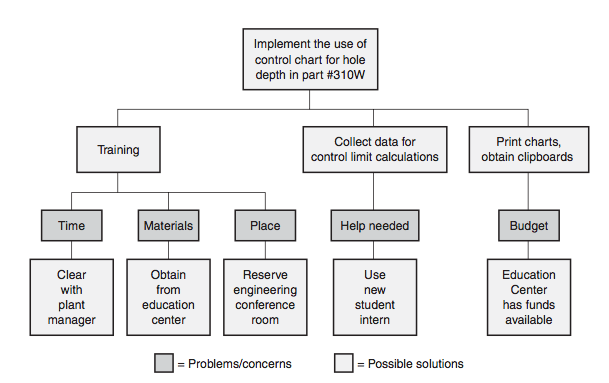
\includegraphics[width=120mm]{imagenes/PDPC.png}
	\caption{PDPC}
	\label{fig:PDPC}
\end{figure}

Diagrama de árbol para ilustrar problemas, anticiparse a ellos y listar soluciones posibles.

\subsection{Risk Priority Number}

Calculado de los datos FMEA: severidad, ocurrencia y detección. RPN = S x D x O. RPN ayuda a determinar el potencial riesgo y a ayudar al project team para priorizar los items sobre los que trabajar primero.

\subsection{Sampling Plan}

Hacer muestreos en base a factores: velocidad de la linea, tecnología disponible, numero de personas disponible, expectativa del consumidor, ... 
Consiste en coger un numero de muestras aleatorio que representen al conjunto del lote de fabricación.
Juran dijo que la inspección 100\% es solo el 80\% de efectiva.

\subsection{Diagrama SIPOC}

Definir procesos y sus limites. Identificar los outputs de los procesos, incluyendo datos, servicios, productos, información, registros... Ve a la columna de customers, para saber quien recibe qué output. Vuelve a la columna de Suppliers para identificar cuales son los internos y cuales los externos y cuales son sus inputs.

\subsection{Tree Diagram}

Ayuda a romper el topic genereal en un numero de actividades que contribuyen entre sí. El Team project debe dar entre 2 y 5 topics que contribuyan con el topic general, y la idea es ponerlos en línea horizontal. Se continua la rama del arbol hasta que no sea práctico. Se revisa el arbol consiguiendo seguridad de que trabajar cada item puede mejorar el topic. Por lo que el arbol resultante provee actividades específicas que contribuyen al topic general.

\begin{figure}[ht!]
	\centering
	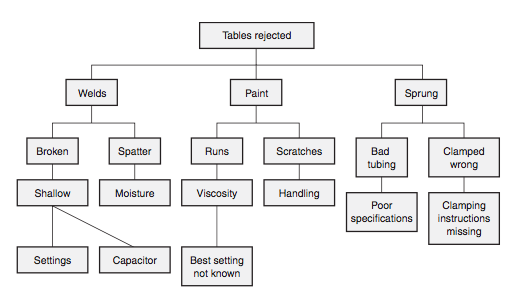
\includegraphics[width=120mm]{imagenes/TreeDiagram.png}
	\caption{Tree Diagram}
	\label{fig:TreeDiagram}
\end{figure}

\subsection{Tool Review}

La fase de definición se centra en determinar el alcance de las mejoras del proyecto y de los recursos y calendario necesitado para ejecutar el proyecto. Hay mucha herramientas para ayudar en la definición y gestión del proyecto, incluyendo Gantt. Las herramientas y el nivel de detalle debe ser basado en el tamaño del proyecto.

\section{Resultados de negocios para Proyectos}

Los resultados de negocios pueden ser mostrados de muchas maneras y en muchos niveles de detalle. Las medidas de los resultados de proyectos deben ser identificadas durante la fase inicial y redefinidas mientras el proyecto avance. Las \textit{performance measures (medidas de desempeño)} estan relacionadas con el negocio, proyectos o procesos y son expresadas a través de \textit{balanced scorecard} o \textit{rendimiento de metas establecidas}.

Por un lado, las \textit{balanced scorecard} requiere que la organización evalúe su actuación en 5 areas princiaples: financiera, cliente, procesos internos, aprendizaje y crecimiento. Así se consigue alinear la visión de la empresa con las metas, asegurando que ningún area sobresalga del resto.

Por otro lado, el rendimiento de las metas establecidas consiste en establecer metas, y revisar la consecución de las mismas a lo largo del tiempo. Siempre deben ser cuantificables. Ejemplo: Incrementar facturación 10\% más sobre el año anterior.

Para medir, se utiliza \textit{Cost performance index (CPI)}, que consiste en establecer un ratio entre el coste/beneficio entre los escenarios actual/futuro. \textit{Schedule performance index (SPI)} mide la eficiencia del calendario también por ratio: objetivos logrados vs planificados.
	
\subsection{Process Performance}

Calcular las métricas \textit{de rendimiento del proceso} como: Defectos por Unidad (DPU), Rolled Throughput Yield (RTY), coste de mala calidad (COPQ), defectos por millón de oportunidades (DPMO), niveles sigma, indices de capacidad de proceso. A través de estas métricas, conduce la toma de decisiones de los proyectos.

La palabra defecto no está permitida ser utilizada relacionada con productos y servicios.

\begin{itemize}
	\item Defects per unit (DPU): número total de defectos dividido por el numero total de productos producidos en un periodo temporal.
	\item Defects per million opportunities (DPMO): calcular el numero de oportunidades, es necesario encontrar el número de caminos que hay para que cada defecto ocurra.
	\item Rolled throughput yield (RTY): RTY aplica al rendimiento desde series de procesos y es encontrado por multiplicidad de procesos individuales.
	\item Sigma levels: Supon la tolerancia de una dimensión en 5 $\pm$ 0.012 [4.988 - 5.012]. Los datos dicen que el proceso es $\sigma = \pm$0.004. 3$\sigma$ caben dentro de tolerancia ya que 3 x $\pm$0.004 = $\pm 12$.
	\item Process capability indices:
	\begin{itemize}
		\item $C_p$: es el ratio de tolerancia $6\sigma$ 
		\item $C_pk$: is the lesser of the USL minus the mean divided by three sigma (or the mean) minus the LSL divided by three sigma. The greater the Cpk value, the better.
		\item $C_r$: el ratio de 1 dividido por $C_p$
	\end{itemize}
\end{itemize}

\subsection{Communication}

Define y describe técnicas de comunicación usadas en la organización: top-down, bottom-up, horizontal.

La transmisión de información implica un cambio del comportamiento, al menos es lo esperado. Es el sentido de comunicar algo en una organización. Es clave que quien dirija tenga buenas habilidades comunicativas, pero todo el mundo las necesita ya que hay diferentes flujos de comunicación.

\begin{itemize}
	\item Top-down flow: Las instrucciones que da el de arriba hacia abajo, la comunicación de las políticas, el feedback de las actuaciones.
	\item Bottom-up flow: desde los operadores de línea a supervisores, encargados y así hacia arriba. Es importante considerar sugerencias.
	\item Horizontal: la mas útil para conseguir resultados rápidos y efectivos. Puede ocurrir que los escalones jerárquicos superiores sientan han sido saltados ya que las decisiones se están arreglando un nivel más abajo entre varios.
\end{itemize}

\section{Team Dynamics and Performance}
\subsection{Team Basics}

There is no 'I' in 'team'. Equipo es un conjunto de esfuerzos individuales. Para aprovechar lo mejor de cada individuo, hay que conocer las fortalezas, roles y responsabilidades de cada uno, así como el alcance de la tarea. ¿Cómo formar un equipo? ¿cómo organizar meetings? ¿cómo gestionar proyectos? ¿como conseguir las metas deseadas. A la hora de comenzar, la idea es marcar las metas, hitos, objetivos y que cada miembro del equipo entienda las expectativas. Generar un orden del día flexible.

En todas las reuniones hay que tener las metas, objetivos y alcance/limites visibles para no perderse.

\subsection{Team Formation}

De 5 a 9 miembros, 7 es el tamaño perfecto, con habilidades complementarias para conseguir metas y objetivos para el equipo. Debe ser conducido por el tamaño y alcance del proyecto. Si se puede, se hacen subdivisiones de proyectos.

El equipo debe incluir expertos y a los grupos de interés. Un proyecto no puede ser implementado si parte de los grupos de interés no están presentes en el desarrollo del mismo.

La interacción es buena, pero puede ser perjudicial. Si hay gran diversidad entre los perfiles, producen mejores interacciones. Los externos suelen hacer preguntas a los que están cerca del proceso. Estos meetings deben ser moderados para no machacar haciendo demasiadas preguntas.

\subsection{Virtual teams}

Innovación debido a las nuevas tecnologías. A través de internet se comparten datos virtualmente y hacemos meetings en videoconferencia. Reduce costos.

\subsection{Team Stages and Dynamics}

Definir y describir las etapas de la evolucion del equipo: forming, storming, norming, performin, adjourning and recognition. Identificar y ayudar a resolver dinamicas negativas: overbearing, dominante, reluctant participant, la aceptación incuestionada de las opiniones como un hecho, pensamienot grupal, feuding, floundering, the rush to accomplishment, attibution, discounts, digresions and tangents.

Los proyectos fallan por falta de trabajo en equipo. Según B.W. Tuckman's las etapas típicas son: forming, storming, norming and performing. Aunque aquí vamos a meter dos mas

\begin{enumerate}
	\item Forming: que los miembros se conozcan. que no sea un grupo inmaduro. que haya sentido de pertenencia al grupo. orgulloso de estar en el grupo. intentar ayudar a los demas. ser positivo ante los discussion topics. no ea una gran carga de trabajo. los miembros orientados hacia metas. miembros entienden roles y responsabilidades. En conjunto, esta fase es como una \textbf{luna de miel}.
	\item Storming: los miembros dan ideas. entendimiento y alcance de los miembros, sus roles y responsabilidades. ideas y empezar a debatir. los desacuerdos ralentizan al grupo. no se saca mucho trabajo adelante. que no haya interacciones negativas, ni completos desacuerdos.
	\item Norming: los miembros deben resolver sus conflictos. los miembros aceptan ideas para avanzar. mucho trabajo sale adelante. empiezan a funcionar como equipo. los miembros empiezan a confiar unos en otros. 
	\item Performing: Equipo efectivo, habilidades complementarias, se crea sinergia. Cada uno hace lo que mejor sabe hacer.
	\item Transitioning/Adjourning: Se disuelve el equipo. Los miembros vuelven a otras actividades de su trabajo. Si el proyecto continua con un alcance adicional, algunos miembros deben ser cambiados. La dinamca cambia y vuelve a las primeras etapas. 
	\item Recognition: reconocer la labor: notas de agradecimiento, email, newsletter, una reunión con todos los empleados, certificados, bonus o un extra de pasta.
\end{enumerate}

\subsubsection{El liderazgo por etapas: Team Leadership}

\begin{enumerate}
	\item Forming (directing): supervision directa, exhibe comportamiento de director. da instrucciones de que hacer cuando, donde y como. escucha el feedback, anima al equipo, explica los roles y responsabilidades, identifica las oportunidades para desarrollar habilidades.
	\item Storming (coaching): supervision directa, exhibe comportamiento de director. empieza comportamiento de ayuda. escucha más al equipo.
	\item Norming (supporting): baja el nivel de comportamiento como director y más de eayuda. anima a tomar decisiones sobre las responsabilidades. Ayuda a mover la actuación de etapa antes de que vuelvan a una etapa anterior .
	\item Performing (delegating): desde que el equipo es maduro, se reduce el nivel de dirección y de soporte en las funciones del día a día. todavía monitoriza las metas y las actuaciones del equipo. Observa cualquier cambio en la dinámica debido a cambios importantes. 
\end{enumerate}

\subsubsection{Negative Team Dynamics}

\begin{itemize}
	\item Overbearing member(s). Pocos hablan, muchos escuchan. Causas: miembros demasiado influyentes. Medidas: round-robin desde el miembro influyente hacia el resto.
	\item Dominant member(s). Reunión caótica, dificil de esuchar o entender. Causas: dominantes interrumpen al resto constantemente. Medidas: Estructurar el orden del día para que todos hablen. Hacer moderación efectiva. Round-robin.
	\item Floundering. El equipo se encuentra en proceso o está actuando de una manera inestable y vacilante. Causas: Falta de direccion de equipo. Miembros abrumados/sobrecargados. Aplazamiento de las decisiones de equipo. Medidas: más dirección en las primeras etapas. El líder debe ser visible durante la reunión y toma de decisiones.
	\item Participante reacio. Falta de participación. Desinterés. Causas: no tiene interes en los resultados de equipo. Está intimidado por otros miembros. Tiene miedo de perder su trabajo u opiniones. Medidas: Los líderes ayudan a los miembros a que activen su participación.
	\item Aceptación incuestionable de opiniones como hechos. Presentación de datos sin análisis. Causas: razones culturales, falta de gestión por hechos. Medidas: pedir datos.
	\item Groupthink. No hay desacuerdos. Dudas expresadas en ambiente privado. Causas: miedo. Medidas: traer gente que no sea del equipo a participar. Cambiar los roles.
	\item Feuding (riñas, reñirse). Baja moral de equipo, bajo progreso. Causas: resolución de conflictos no efectivos. Falta de respeto entre miembros. Medidas: Disciplina. Confrontar en privado. 
	\item Prisa por el logro. Falta de datos. Análisis inconsistente. Causas: Plazos absurdos. Miembros novatos buscando metas a corto plazo. Medidas: Datos, análisis y significado estadistico. Pedir alternativas. Revisar plazos.
	\item Attribution. miembros hacen referencias casuales. no buscan explicaciones. se dejan llevar por las emociones. Causas: igual que Prisa por el logro. Medidas: Poner en tela de juicio lo que han dicho.
	\item Discounts. Opiniones ignoradas. No se escuchan. Sarcasmo. Medidas: alentar el respeto. preguntar por la clarificación de las opiniones.
	\item Disgressions and tangents. Discusión fuera del alcance. Distracciones. Causas: Cuestiones culturales, falta de liderazgo. Medidas: Hacer cumplir la agenda. 
\end{itemize}

\subsection{Team Roles and Responsibilities}

\begin{tabular}{|c|c|c|c|}
	\hline Rol & Candidato & Training/Background & Responsabilidades principales \\ 
	\hline Executive sponsor & Lider responsable de la unidad de negocio para beneficios y perdidas (de nivel de director o superior) & Conceptos six sigma, overview, definición de operaciones. & Fijar direccion y prioridades para la organizacion Six sigma. Asignar los recursos de los proyectos. Fijar la visión six sigma. Monitorizar el progreso sobre el programa completo. Iniciar programas de incentivos. Recompensar los proyectos exitosos.  \\ 
	\hline Champion & Managers de nivel superior & Conceptos Six Sigma, estrategias, herramientas y métodos, operaciones. Especial énfasis en herramientas de gestión. & Asignar recursos a proyectos. Determinar el criterio para la selección de proyectos. Quitar barreras ocultas para el exito del proyecto. Aprobar el proyecto completo. Implementar cambios. \\ 
	\hline Process Owner & Persona responsable y que controle la ejecución y resultados del proceso. Sponsor o Champion puede ser este perfil al mismo tiempo. & Conceptos Six Sigma, estrategias, herramientas, metodología, definiciones. & Selecionar team members. Asignar recursos a proyectos. Proveer conocimiento del proceso. Revisar cambios del proceso. Aprobar cambios. Implementar cambios. Asegurar que las mejoras son sustanciales. \\ 
	\hline 
\end{tabular} 

\end{document}
